\documentclass{article}
\title{ECE 370 -- Homework 5}
\usepackage[margin=1in]{geometry}
\usepackage{graphicx}
\usepackage{pdfpages}
\usepackage{fancyhdr}
\usepackage{enumitem}
\usepackage{pdfpages}
\usepackage{amsmath}
\usepackage{amssymb}
\usepackage{float}
\pagestyle{fancy}
\fancyhf{}
\fancyhead[L]{Gianni Avilan-Losee}
\fancyhead[C]{ECE 370}
\fancyhead[R]{Homework 5}
\fancyfoot[C]{\thepage}
\usepackage{microtype}
\usepackage{textcomp, gensymb}
\author{Gianni Avilan-Losee}
\setcounter{section}{1}
\begin{document}
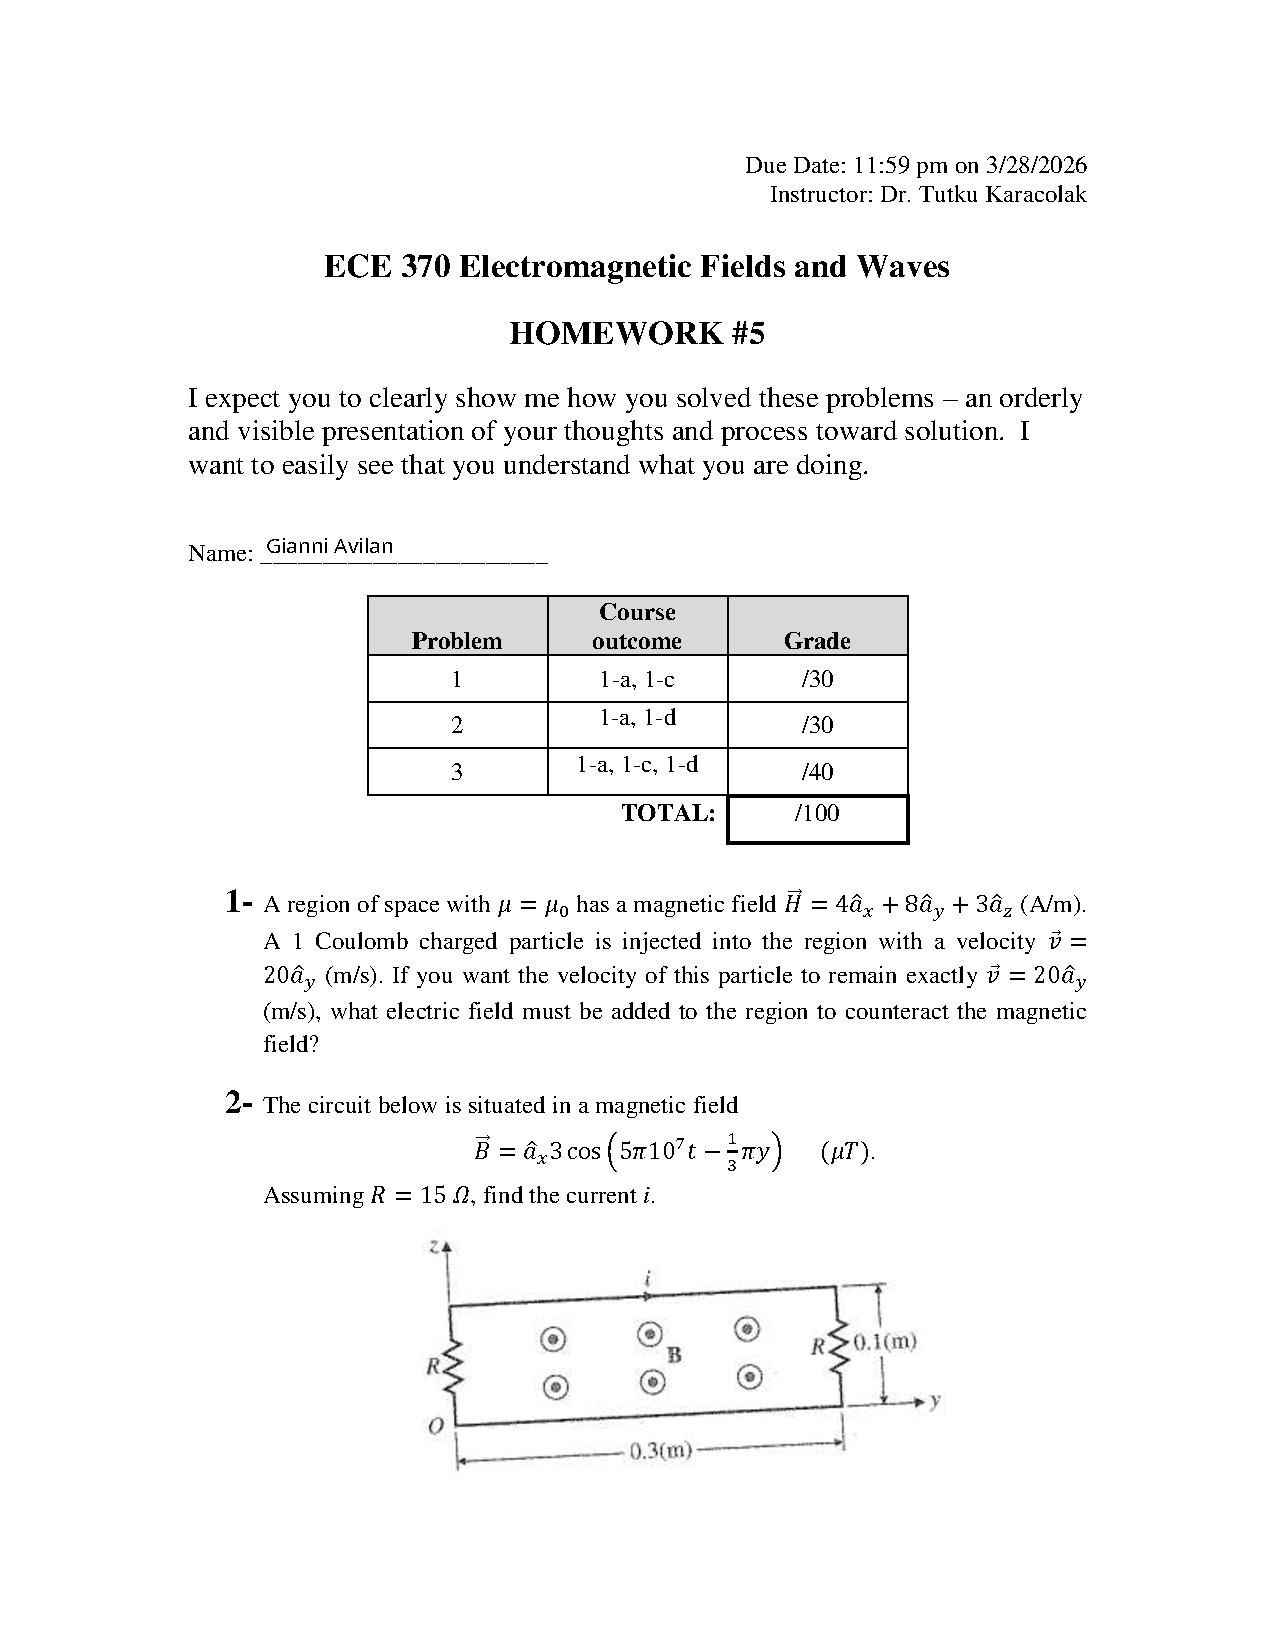
\includepdf[pages=-]{homework-5_cover-page.pdf}
\begin{enumerate}
	\item Given that the total force induced by the electric and magnetic fields is equal to the sum of the individual force induced by each field, 
		\[
			\vec{F} = \vec{F}_e + \vec{F}_m = q(\vec{E} + \vec{u} \times \vec{B}),
		\]
		we may solve for \(\vec{E}\), the electric field intensity necessary for the particle to maintain a constant speed with no acceleration, by assuming a net zero force on the particle, \(F =0\). Since we know the magnetic field intensity, \(\vec{H}\), we may derive the magnetic flux density \(\vec{B}\) as 
		\[
			\vec{B} = \mu_0 \vec{H} = \mu_0[4 \hat{x} + 8 \hat{y} + 3 \hat{z}]^{\mathrm{T}}.
		\]
		Solving for \(\vec{E}\),
		\begin{align*}
			\vec{E} &= -(20 \hat{y} \times \mu_0[4 \hat{x} + 8 \hat{y} + 3 \hat{z}]) \\
							&=(20)(9.434)\sin{(\theta)} \ \hat{n},
		\end{align*}
		where \(\theta\) is the angle between the two vectors and \(\hat{n}\) is the normal vector, whose direction is determined with the right-hand rule. We may find the angle using the dot product of the unit vectors \(\hat{u}\) and \(\hat{y}\), as 
		\[
			\theta = \cos^{-1}{(\hat{y} \cdot \hat{u})} = \cos^{-1}\left(\frac{8}{9.434}\right) = 0.5586 = 32.01\degree,
		\]
		and so 
		\[
			\vec{E} = -(\vec{u} \times \vec{B}) = -188.68 \sin{(32.01\degree)} = -\hat{n} \ 100\mu_0.
		\]
		To determine the direction of the normal vector, we may use the determinant definition of the cross product, so that
		\[
			\vec{E} = -\det\begin{bmatrix}
				\hat{x} & \hat{y} & \hat{z} \\
				0 & 20 & 0 \\
				4 & 8 & 3 \\
			\end{bmatrix} = -\hat{x}60 + \hat{z} 80,
		\]
		and so 
		\[
			\vec{E} = (-\hat{x}60 + \hat{y}80)\mu_0 = -\hat{x}[7.54 \times 10^{-5}] + \hat{z}[10^{-4}] \ \mathrm{\frac{V}{m}}.
		\]

	\item Using the formula for transformer emf, 
		\[
			V^{\mathrm{tr}}_{\mathrm{emf}} = -N\int_S \frac{\partial \vec{B}}{\partial t} \cdot d \vec{s},
		\]
		we begin by assuming \(N = 1\) and then proceed to solve for \(\frac{\partial \vec{B}}{\partial t}\) as
		\[
			\frac{\partial \vec{B}}{\partial t} = \frac{\partial }{\partial t} \hat{x} \ 3\cos{(5\pi 10^7t-\frac{1}{3}\pi y)} = -\hat{x}15\pi10^7t\sin{(5\pi 10^7 t - \frac{1}{3}\pi y)} \ \mathrm{\frac{\micro T}{s}}.
		\]
		Then, aliging the differential surface vector of the loop \(d \vec{s}\) with the direction of \(\vec{B}\) (the choice between the two possible normal vectors is arbitrary, but this choice aligns the resulting potential difference with the direction of the resultant curret) we may express \(d \vec{s}\) as
		\[
		  d \vec{s} = \hat{x} \ dz \ dy.
		\]

		Substituting into the equation for \(V_{\mathrm{emf}}^{\mathrm{tr}}\) and using the height and width of the loop as the bounds of integration,
		\begin{align*}
			V_{\mathrm{emf}}^{\mathrm{tf}} &= -\int_{0}^{0.3} \int_{0}^{0.1} -\hat{x}15\pi10^7\sin{(5\pi 10^7 t - \frac{1}{3}\pi y)} \cdot \hat{x} \ dz \ dy \\
																		 &= \int_{0}^{0.3} \int_{0}^{0.1} 15\pi 10^7\sin{(5\pi10^7t-\frac{1}{3}\pi y)} \ dz \ dy \\
																		 &= \int_{0}^{0.3} 15\pi10^6\sin{(5\pi10^7t-\frac{1}{3}\pi y)} \ dy \\
																		 &=15\pi10^6 \ [\frac{3}{\pi}\cos{(5\pi10^7 t - \frac{\pi}{3} y)} \ \biggr\rvert_{0}^{0.3}] \\
																		 &=45 \times 10^6 \ [\cos{(1.57 \times 10^8t -0.3142)} - \cos{(1.57 \times 10^8t)}] \ \mathrm{\micro V} \\
																		 &=45 \ [\cos{(1.57\times10^8t - 0.3142) - \cos{(1.57 \times 10^8 t)}}] \ \mathrm{V}.
		\end{align*}

		To find current \(i\), we may use Ohm's Law and simplify the cosine terms,
		\[
			i = \frac{V_{\mathrm{emf}}^{\mathrm{tf}}}{2R} = \frac{45}{30} \ [\cos{(1.57 \times 10^8t - 0.3142)} - \cos{(1.57\times10^8t)}] \ \mathrm{A}
		\]
		with the resulting current flowing in the clockwise direction.

		\item
			\begin{enumerate}[label=\alph*)]
				\item Here, we have another stationary, conducting loop in a time-varying magnetic field induced by a coplanar current-carrying wire. Again using the formula for \(V_{\mathrm{emf}}^{\mathrm{tf}}\) and assuming \(N=1\), we may first express the magnetic field induced by a current-carrying wire as
					\[
						\vec{B} = \frac{\mu_0I}{2\pi R} \ \mathrm{T}.
					\]
					Considering that the current in the wire is time-varying and considering the radial distance from the wire in the \(x\) direction, we may formulate the magnetic flux density induced by \textit{this} wire as
					\[
						\vec{B} = \hat{y} \ \frac{\mu_0I_o\cos{(\omega t)}}{2\pi x} \ \mathrm{T}
					\]
					and its time derivative as
					\[
						\frac{\partial \vec{B}}{\partial t} = \hat{y} \frac{\mu_0 I_0}{2\pi x}\frac{\partial }{\partial t}cos{(\omega t)} = -\hat{y} \ \frac{\mu_0 I_0 \omega}{2 \pi x}\sin{(\omega t)} \ \mathrm{\frac{T}{s}}.
					\]
			Then, \(d \vec{s}\) may be formulated (in the same direction as \(\vec{B}\)) as 
			\[
			  d \vec{s} = \hat{y} \ dx \ dz.
			\]

			Putting everything together, 
			\[
				V_{\mathrm{emf}}^{\mathrm{tf}} = \int_{S} \left[ \hat{y} \ \frac{\mu_0 I_0 \omega}{2 \pi x} \sin{(\omega t)}\right] \cdot \left[\hat{y} \ dx \ dz \right].
			\]
			Simplifing and pulling out constants,
			\[
				V^{\mathrm{tf}}_{\mathrm{emf}} = \frac{\mu_0 I_0 \omega \sin{(\omega t)}}{2\pi} \int_S \frac{1}{x} \ dx \ dz = \frac{\mu_0 I_0 \omega \sin{(\omega t)}}{2\pi} \int_{0}^{a} \int_{x_0}^{x_0 + b} \frac{1}{x} \ dx \ dz.
			\]
			Solving, 
			\[
				V_{\mathrm{emf}}^{\mathrm{tf}} = \frac{\mu_0 I_0 \omega \sin{(\omega t)}}{2\pi} \left[ a\ln\left(\frac{x_0 + b}{x_0}\right)\right] \ \mathrm{V},
			\]
			with current flowing in the counter-clockwise direction.
			\item
				Here, we may integrate each side of the rectangular loop separately to find the induced motional EMF, \(V_{\mathrm{emf}}^{\mathrm{m}}\), in the loop. Motional EMF induced by a static magnetic field \(\vec{B}\) is given by
				\[
					V_{\mathrm{emf}}^{\mathrm{m}} = \oint_C (\vec{u} \times \vec{B}) \cdot d \vec{l}.
				\]
				Integrating to first find the voltage difference across the horizontal bottom segment of the loop, 
				\[
				  \int_{x_0}^{(x_o+b)} \left(\hat{x} \ u_0 \times \hat{y} \ \frac{\mu_0 I}{2 \pi R}\right) \cdot \hat{x} \ dl.
				\]
				Since \(\hat{x} \times \hat{y} = \hat{z}\) and \(\hat{z} \cdot \hat{x} = 0\), we may assume that there is no voltage difference induced across the horizontal bottom segment of the loop, and likewise for the horizontal top section.

				Then, finding the motional emf induced across the right-hand vertical segment of the loop,
				\[
					\int_{0}^{a}\left(\hat{x} \ u_0 \times \hat{y} \ \frac{\mu_0 I}{2 \pi R} \right) \cdot \hat{z} \ dl = \int_{0}^{a}\hat{z} \ \frac{u_0\mu_0I}{2 \pi R} \cdot \hat{z} \ dl = \int_{0}^{a} \frac{u_0\mu_0I}{2\pi R} = \frac{au_0\mu_0I}{2\pi R} \ \mathrm{V}.
				\]
				Evaluating the left-hand vertical segment of the loop will result in 
				\[
					\int_{a}^{0}\frac{u_0\mu_0 I}{2\pi R} = -\frac{au_0\mu_0 I}{2\pi R} \ \mathrm{V}.
				\]
				Assuming the radial distance between the vertical conducting wire and the conducting loop is measured from the left-hand side of the conducting loop, we may then express the total induced voltage in the loop as 
				\[
					-\frac{au_0\mu_0I}{2 \pi R} + \frac{au_0\mu_0 I}{2\pi (R+b)} \ \mathrm{V},
				\]
				with current flowing in the counter-clockwise direction (assuming some resistance in the loop).
			\item Since total induced emf is the sum of transformer and motional emf,
				\[
					V_{\mathrm{emf}} = \frac{\mu_0I\omega\sin{(\omega t)}}{2\pi}\left[a \ln{\left(\frac{x_0 + b}{x_0}\right)}\right] - \frac{au_0\mu_0I}{2\pi R} + \frac{au_0\mu_0I}{2\pi(R+b)} \ \mathrm{V}.
				\]
		\end{enumerate}
\end{enumerate}
\end{document}
